\documentclass{standalone}
\usepackage{pgfplots}
\pgfplotsset{compat=1.18}
\usetikzlibrary{calc}
\usetikzlibrary{arrows.meta}

\begin{document}

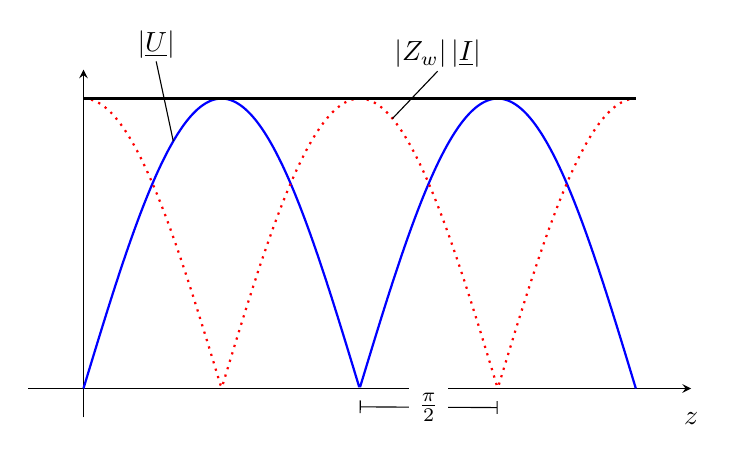
\begin{tikzpicture}

\begin{axis}[
    axis lines=middle,
    xlabel={$z$},
    xlabel style={below=5pt},
    ylabel={},
    xtick=\empty,
    ytick=\empty,
    domain=0:2*pi,
    samples=400,
    width=10cm,
    height=6cm,
    enlargelimits
    ]
    \addplot [thick, blue] {abs(sin(deg(x)))} node[pos=0.175] (A) {} node[pos=0.5, below] (E1) {};
    \addplot [thick, red, dotted] {abs(cos(deg(x)))} node[pos=0.55] (C) {} node[pos=0.75, below] (E2) {};
    \addplot [thick, black] {1};

\end{axis}

% annotation for voltage
\node[inner sep=1pt] (B) at ($(A) + (100:1.25cm)$) {$|\underline{U}|$};
\draw (A.center) -- (B.south);

% annotation for current
\node[inner sep=1pt] (D) at ($(C) + (55:1cm)$) {$|Z_{w}| \, |\underline{I}|$};
\draw (C.center) -- (D.south);

% pahse shift
\draw[|-|] (E1.south) -- (E2.south) node[fill=white, pos=0.5] {$\frac{\pi}{2}$};

\end{tikzpicture}

\end{document}